\documentclass{sigchi}

% Use this section to set the ACM copyright statement (e.g. for
% preprints).  Consult the conference website for the camera-ready
% copyright statement.

% Copyright
\CopyrightYear{2016}
%\setcopyright{acmcopyright}
\setcopyright{acmlicensed}
%\setcopyright{rightsretained}
%\setcopyright{usgov}
%\setcopyright{usgovmixed}
%\setcopyright{cagov}
%\setcopyright{cagovmixed}
% DOI
\doi{http://dx.doi.org/10.475/123_4}
% ISBN
\isbn{123-4567-24-567/08/06}
%Conference
\conferenceinfo{CHI'16,}{May 07--12, 2016, San Jose, CA, USA}
%Price
\acmPrice{\$15.00}

% Use this command to override the default ACM copyright statement
% (e.g. for preprints).  Consult the conference website for the
% camera-ready copyright statement.

%% HOW TO OVERRIDE THE DEFAULT COPYRIGHT STRIP --
%% Please note you need to make sure the copy for your specific
%% license is used here!
% \toappear{
% Permission to make digital or hard copies of all or part of this work
% for personal or classroom use is granted without fee provided that
% copies are not made or distributed for profit or commercial advantage
% and that copies bear this notice and the full citation on the first
% page. Copyrights for components of this work owned by others than ACM
% must be honored. Abstracting with credit is permitted. To copy
% otherwise, or republish, to post on servers or to redistribute to
% lists, requires prior specific permission and/or a fee. Request
% permissions from \href{mailto:Permissions@acm.org}{Permissions@acm.org}. \\
% \emph{CHI '16},  May 07--12, 2016, San Jose, CA, USA \\
% ACM xxx-x-xxxx-xxxx-x/xx/xx\ldots \$15.00 \\
% DOI: \url{http://dx.doi.org/xx.xxxx/xxxxxxx.xxxxxxx}
% }

% Arabic page numbers for submission.  Remove this line to eliminate
% page numbers for the camera ready copy
% \pagenumbering{arabic}

% Load basic packages
\usepackage{balance}       % to better equalize the last page
\usepackage{graphics}      % for EPS, load graphicx instead
\usepackage[T1]{fontenc}   % for umlauts and other diaeresis
\usepackage{txfonts}
\usepackage{mathptmx}
\usepackage[pdflang={en-US},pdftex]{hyperref}
\usepackage{color}
\usepackage{booktabs}
\usepackage{textcomp}

% Some optional stuff you might like/need.
\usepackage{microtype}        % Improved Tracking and Kerning
% \usepackage[all]{hypcap}    % Fixes bug in hyperref caption linking
\usepackage{ccicons}          % Cite your images correctly!
% \usepackage[utf8]{inputenc} % for a UTF8 editor only

% If you want to use todo notes, marginpars etc. during creation of
% your draft document, you have to enable the "chi_draft" option for
% the document class. To do this, change the very first line to:
% "\documentclass[chi_draft]{sigchi}". You can then place todo notes
% by using the "\todo{...}"  command. Make sure to disable the draft
% option again before submitting your final document.
\usepackage{todonotes}

% Paper metadata (use plain text, for PDF inclusion and later
% re-using, if desired).  Use \emtpyauthor when submitting for review
% so you remain anonymous.
\def\plaintitle{SIGCHI Conference Proceedings Format}
\def\plainauthor{First Author, Second Author, Third Author,
  Fourth Author, Fifth Author, Sixth Author}
\def\emptyauthor{}
\def\plainkeywords{Authors' choice; of terms; separated; by
  semicolons; include commas, within terms only; required.}
\def\plaingeneralterms{Documentation, Standardization}

% llt: Define a global style for URLs, rather that the default one
\makeatletter
\def\url@leostyle{%
  \@ifundefined{selectfont}{
    \def\UrlFont{\sf}
  }{
    \def\UrlFont{\small\bf\ttfamily}
  }}
\makeatother
\urlstyle{leo}

% To make various LaTeX processors do the right thing with page size.
\def\pprw{8.5in}
\def\pprh{11in}
\special{papersize=\pprw,\pprh}
\setlength{\paperwidth}{\pprw}
\setlength{\paperheight}{\pprh}
\setlength{\pdfpagewidth}{\pprw}
\setlength{\pdfpageheight}{\pprh}

% Make sure hyperref comes last of your loaded packages, to give it a
% fighting chance of not being over-written, since its job is to
% redefine many LaTeX commands.
\definecolor{linkColor}{RGB}{6,125,233}
\hypersetup{%
  pdftitle={\plaintitle},
% Use \plainauthor for final version.
%  pdfauthor={\plainauthor},
  pdfauthor={\emptyauthor},
  pdfkeywords={\plainkeywords},
  pdfdisplaydoctitle=true, % For Accessibility
  bookmarksnumbered,
  pdfstartview={FitH},
  colorlinks,
  citecolor=black,
  filecolor=black,
  linkcolor=black,
  urlcolor=linkColor,
  breaklinks=true,
  hypertexnames=false
}

% create a shortcut to typeset table headings
% \newcommand\tabhead[1]{\small\textbf{#1}}

% End of preamble. Here it comes the document.
\begin{document}

\title{\plaintitle}

\numberofauthors{3}
\author{%
  \alignauthor{Leave Authors Anonymous\\
    \affaddr{for Submission}\\
    \affaddr{City, Country}\\
    \email{e-mail address}}\\
  \alignauthor{Leave Authors Anonymous\\
    \affaddr{for Submission}\\
    \affaddr{City, Country}\\
    \email{e-mail address}}\\
  \alignauthor{Leave Authors Anonymous\\
    \affaddr{for Submission}\\
    \affaddr{City, Country}\\
    \email{e-mail address}}\\
}

\maketitle

\begin{abstract}
  UPDATED---\today. This sample paper describes the formatting
  requirements for SIGCHI conference proceedings, and offers
  recommendations on writing for the worldwide SIGCHI
  readership. Please review this document even if you have submitted
  to SIGCHI conferences before, as some format details have changed
  relative to previous years. Abstracts should be about 150 words and
  are required.
\end{abstract}

\category{H.5.m.}{Information Interfaces and Presentation
  (e.g. HCI)}{Miscellaneous} \category{See
  \url{http://acm.org/about/class/1998/} for the full list of ACM
  classifiers. This section is required.}{}{}

\keywords{\plainkeywords}

\section{Introduction}

This format is to be used for submissions that are published in the
conference proceedings. We wish to give this volume a consistent,
high-quality appearance. We therefore ask that authors follow some
simple guidelines. You should format your paper exactly like this
document. The easiest way to do this is to replace the content with
your own material.  This document describes how to prepare your
submissions using \LaTeX.

\section{Page Size and Columns}
On each page your material should fit within a rectangle of 7 $\times$
9.15 inches (18 $\times$ 23.2 cm), centered on a US Letter page (8.5
$\times$ 11 inches), beginning 0.85 inches (1.9 cm) from the top of
the page, with a 0.3 inches (0.85 cm) space between two 3.35 inches
(8.4 cm) columns. Right margins should be justified, not
ragged. Please be sure your document and PDF are US letter and not A4.

\section{Typeset Text}
The styles contained in this document have been modified from the
default styles to reflect ACM formatting conventions. For example,
content paragraphs like this one are formatted using the Normal style.

\LaTeX\ sometimes will create overfull lines that extend into columns.
To attempt to combat this, the \texttt{.cls} file has a command,
\texttt{{\textbackslash}sloppy}, that essentially asks \LaTeX\ to
prefer underfull lines with extra whitespace.  For more details on
this, and info on how to control it more finely, check out
{\url{http://www.economics.utoronto.ca/osborne/latex/PMAKEUP.HTM}}.

\subsection{Title and Authors}

Your paper's title, authors and affiliations should run across the
full width of the page in a single column 17.8 cm (7 in.) wide.  The
title should be in Helvetica or Arial 18-point bold.  Authors' names
should be in Times New Roman or Times Roman 12-point bold, and
affiliations in 12-point regular.

See \texttt{{\textbackslash}author} section of this template for
instructions on how to format the authors. For more than three
authors, you may have to place some address information in a footnote,
or in a named section at the end of your paper. Names may optionally
be placed in a single centered row instead of at the top of each
column. Leave one 10-point line of white space below the last line of
affiliations.

\subsection{Abstract and Keywords}

Every submission should begin with an abstract of about 150 words,
followed by a set of Author Keywords and ACM Classification
Keywords. The abstract and keywords should be placed in the left
column of the first page under the left half of the title. The
abstract should be a concise statement of the problem, approach, and
conclusions of the work described. It should clearly state the paper's
contribution to the field of HCI\@.

\subsection{Normal or Body Text}

Please use a 10-point Times New Roman or Times Roman font or, if this
is unavailable, another proportional font with serifs, as close as
possible in appearance to Times Roman 10-point. Other than Helvetica
or Arial headings, please use sans-serif or non-proportional fonts
only for special purposes, such as source code text.

\subsection{First Page Copyright Notice}
This template include a sample ACM copyright notice at the bottom of
page 1, column 1.  Upon acceptance, you will be provided with the
appropriate copyright statement and unique DOI string for publication.
Accepted papers will be distributed in the conference
publications. They will also be placed in the ACM Digital Library,
where they will remain accessible to thousands of researchers and
practitioners worldwide. See
\url{http://acm.org/publications/policies/copyright_policy} for the
ACM's copyright and permissions policy.

\subsection{Subsequent Pages}

On pages beyond the first, start at the top of the page and continue
in double-column format.  The two columns on the last page should be
of equal length.

\begin{figure}
\centering
  
\includegraphics[width=0.9\columnwidth]{../figures/sigchi-logo}
  \caption{Insert a caption below each figure. Do not alter the
    Caption style.  One-line captions should be centered; multi-line
    should be justified. }~\label{fig:figure1}
\end{figure}

\subsection{References and Citations}

Use a numbered list of references at the end of the article, ordered
alphabetically by last name of first author, and referenced by numbers
in
brackets~\cite{acm_categories,ethics,Klemmer:2002:WSC:503376.503378}.
Your references should be published materials accessible to the
public. Internal technical reports may be cited only if they are
easily accessible (i.e., you provide the address for obtaining the
report within your citation) and may be obtained by any reader for a
nominal fee. Proprietary information may not be cited. Private
communications should be acknowledged in the main text, not referenced
(e.g., ``[Borriello, personal communication]'').

References should be in ACM citation format:
\url{http://acm.org/publications/submissions/latex_style}. This
includes citations to internet
resources~\cite{acm_categories,cavender:writing,CHINOSAUR:venue,psy:gangnam}
according to ACM format, although it is often appropriate to include
URLs directly in the text, as above.


% Use a numbered list of references at the end of the article, ordered
% alphabetically by first author, and referenced by numbers in
% brackets~\cite{ethics, Klemmer:2002:WSC:503376.503378,
%   Mather:2000:MUT, Zellweger:2001:FAO:504216.504224}. For papers from
% conference proceedings, include the title of the paper and an
% abbreviated name of the conference (e.g., for Interact 2003
% proceedings, use \textit{Proc. Interact 2003}). Do not include the
% location of the conference or the exact date; do include the page
% numbers if available. See the examples of citations at the end of this
% document. Within this template file, use the \texttt{References} style
% for the text of your citation.

% Your references should be published materials accessible to the
% public.  Internal technical reports may be cited only if they are
% easily accessible (i.e., you provide the address for obtaining the
% report within your citation) and may be obtained by any reader for a
% nominal fee.  Proprietary information may not be cited. Private
% communications should be acknowledged in the main text, not referenced
% (e.g., ``[Robertson, personal communication]'').

\begin{table}
  \centering
  \begin{tabular}{l r r r}
    % \toprule
    & & \multicolumn{2}{c}{\small{\textbf{Test Conditions}}} \\
    \cmidrule(r){3-4}
    {\small\textit{Name}}
    & {\small \textit{First}}
      & {\small \textit{Second}}
    & {\small \textit{Final}} \\
    \midrule
    Marsden & 223.0 & 44 & 432,321 \\
    Nass & 22.2 & 16 & 234,333 \\
    Borriello & 22.9 & 11 & 93,123 \\
    Karat & 34.9 & 2200 & 103,322 \\
    % \bottomrule
  \end{tabular}
  \caption{Table captions should be placed below the table. We
    recommend table lines be 1 point, 25\% black. Minimize use of
    table grid lines.}~\label{tab:table1}
\end{table}

\section{Sections}

The heading of a section should be in Helvetica or Arial 9-point bold,
all in capitals. Sections should \textit{not} be numbered.

\subsection{Subsections}

Headings of subsections should be in Helvetica or Arial 9-point bold
with initial letters capitalized.  For sub-sections and
sub-subsections, a word like \emph{the} or \emph{of} is not
capitalized unless it is the first word of the heading.

\subsubsection{Sub-subsections}

Headings for sub-subsections should be in Helvetica or Arial 9-point
italic with initial letters capitalized.  Standard
\texttt{{\textbackslash}section}, \texttt{{\textbackslash}subsection},
and \texttt{{\textbackslash}subsubsection} commands will work fine in
this template.

\section{Figures/Captions}

Place figures and tables at the top or bottom of the appropriate
column or columns, on the same page as the relevant text (see
Figure~\ref{fig:figure1}). A figure or table may extend across both
columns to a maximum width of 17.78 cm (7 in.).

\begin{figure*}
  \centering
  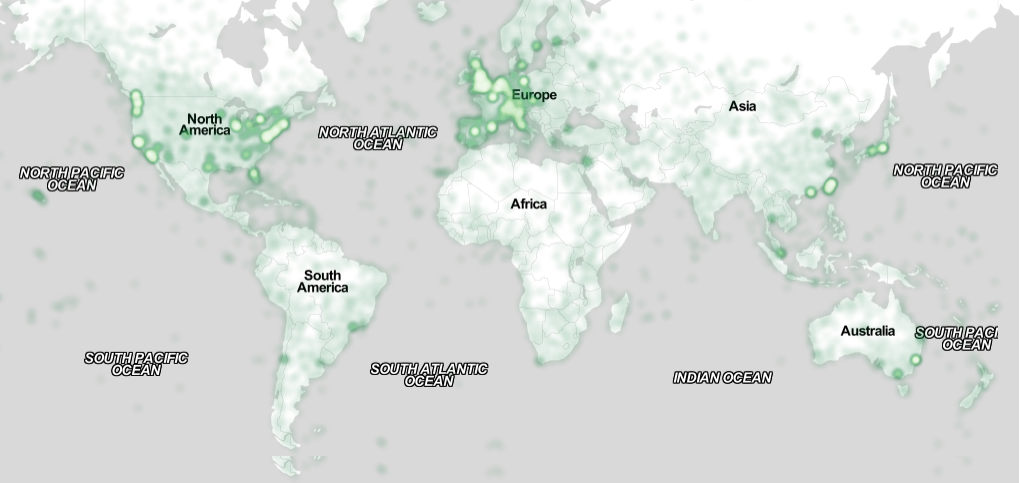
\includegraphics[width=1.75\columnwidth]{../figures/map}
  \caption{In this image, the map maximizes use of space. You can make
    figures as wide as you need, up to a maximum of the full width of
    both columns. Note that \LaTeX\ tends to render large figures on a
    dedicated page. Image: \ccbynd~ayman on
    Flickr.}~\label{fig:figure2}
\end{figure*}

Captions should be Times New Roman or Times Roman 9-point bold.  They
should be numbered (e.g., ``Table~\ref{tab:table1}'' or
``Figure~\ref{fig:figure1}''), centered and placed beneath the figure
or table.  Please note that the words ``Figure'' and ``Table'' should
be spelled out (e.g., ``Figure'' rather than ``Fig.'') wherever they
occur. Figures, like Figure~\ref{fig:figure2}, may span columns and
all figures should also include alt text for improved accessibility.
Papers and notes may use color figures, which are included in the page
limit; the figures must be usable when printed in black-and-white in
the proceedings.

The paper may be accompanied by a short video figure up to five
minutes in length. However, the paper should stand on its own without
the video figure, as the video may not be available to everyone who
reads the paper.

\subsection{Inserting Images}
When possible, include a vector formatted graphic (i.e. PDF or EPS).
When including bitmaps,  use an image editing tool to resize the image
at the appropriate printing resolution (usually 300 dpi).

\section{Quotations}
Quotations may be italicized when \textit{``placed inline''} (Anab,
23F).

\begin{quote}
Longer quotes, when placed in their own paragraph, need not be
italicized or in quotation marks when indented (Ramon, 39M).
\end{quote}

\section{Language, Style, and Content}

The written and spoken language of SIGCHI is English. Spelling and
punctuation may use any dialect of English (e.g., British, Canadian,
US, etc.) provided this is done consis- tently. Hyphenation is
optional. To ensure suitability for an international audience, please
pay attention to the following:

\begin{itemize}
\item Write in a straightforward style.
\item Try to avoid long or complex sentence structures.
\item Briefly define or explain all technical terms that may be
  unfamiliar to readers.
\item Explain all acronyms the first time they are used in your
  text---e.g., ``Digital Signal Processing (DSP)''.
\item Explain local references (e.g., not everyone knows all city
  names in a particular country).
\item Explain ``insider'' comments. Ensure that your whole audience
  understands any reference whose meaning you do not describe (e.g.,
  do not assume that everyone has used a Macintosh or a particular
  application).
\item Explain colloquial language and puns. Understanding phrases like
  ``red herring'' may require a local knowledge of English.  Humor and
  irony are difficult to translate.
\item Use unambiguous forms for culturally localized concepts, such as
  times, dates, currencies, and numbers (e.g., ``1--5--97'' or
  ``5/1/97'' may mean 5 January or 1 May, and ``seven o'clock'' may
  mean 7:00 am or 19:00). For currencies, indicate equivalences:
  ``Participants were paid {\fontfamily{txr}\selectfont \textwon}
  25,000, or roughly US \$22.''
\item Be careful with the use of gender-specific pronouns (he, she)
  and other gendered words (chairman, manpower, man-months). Use
  inclusive language that is gender-neutral (e.g., she or he, they,
  s/he, chair, staff, staff-hours, person-years). See the
  \textit{Guidelines for Bias-Free Writing} for further advice and
  examples regarding gender and other personal
  attributes~\cite{Schwartz:1995:GBF}. Be particularly aware of
  considerations around writing about people with disabilities.
\item If possible, use the full (extended) alphabetic character set
  for names of persons, institutions, and places (e.g.,
  Gr{\o}nb{\ae}k, Lafreni\'ere, S\'anchez, Nguy{\~{\^{e}}}n,
  Universit{\"a}t, Wei{\ss}enbach, Z{\"u}llighoven, \r{A}rhus, etc.).
  These characters are already included in most versions and variants
  of Times, Helvetica, and Arial fonts.
\end{itemize}

\section{Accessibility}
The Executive Council of SIGCHI has committed to making SIGCHI
conferences more inclusive for researchers, practitioners, and
educators with disabilities. As a part of this goal, the all authors
are asked to work on improving the accessibility of their
submissions. Specifically, we encourage authors to carry out the
following five steps:
\begin{enumerate}
\item Add alternative text to all figures
\item Mark table headings
\item Add tags to the PDF
\item Verify the default language
\item Set the tab order to ``Use Document Structure''
\end{enumerate}
For more information and links to instructions and resources, please
see: \url{http://chi2016.acm.org/accessibility}.  The
\texttt{{\textbackslash}hyperref} package allows you to create well tagged PDF files,
please see the preamble of this template for an example.

\section{Page Numbering, Headers and Footers}
Your final submission should not contain footer or header information
at the top or bottom of each page. Specifically, your final submission
should not include page numbers. Initial submissions may include page
numbers, but these must be removed for camera-ready. Page numbers will
be added to the PDF when the proceedings are assembled.

\section{Producing and Testing PDF Files}

We recommend that you produce a PDF version of your submission well
before the final deadline.  Your PDF file must be ACM DL
Compliant. The requirements for an ACM Compliant PDF are available at:
{\url{http://www.sheridanprinting.com/typedept/ACM-distilling-settings.htm}}.

Test your PDF file by viewing or printing it with the same software we
will use when we receive it, Adobe Acrobat Reader Version 10. This is
widely available at no cost. Note that most
reviewers will use a North American/European version of Acrobat
reader, so please check your PDF accordingly.

When creating your PDF from Word, ensure that you generate a tagged
PDF from improved accessibility. This can be done by using the Adobe
PDF add-in, also called PDFMaker. Select Acrobat | Preferences from
the ribbon and ensure that ``Enable Accessibility and Reflow with
tagged Adobe PDF'' is selected. You can then generate a tagged PDF by
selecting ``Create PDF'' from the Acrobat ribbon.

\section{Conclusion}

It is important that you write for the SIGCHI audience. Please read
previous years' proceedings to understand the writing style and
conventions that successful authors have used. It is particularly
important that you state clearly what you have done, not merely what
you plan to do, and explain how your work is different from previously
published work, i.e., the unique contribution that your work makes to
the field. Please consider what the reader will learn from your
submission, and how they will find your work useful. If you write with
these questions in mind, your work is more likely to be successful,
both in being accepted into the conference, and in influencing the
work of our field.

\section{Acknowledgments}

Sample text: We thank all the volunteers, and all publications support
and staff, who wrote and provided helpful comments on previous
versions of this document. Authors 1, 2, and 3 gratefully acknowledge
the grant from NSF (\#1234--2012--ABC). \textit{This whole paragraph is
  just an example.}

% Balancing columns in a ref list is a bit of a pain because you
% either use a hack like flushend or balance, or manually insert
% a column break.  http://www.tex.ac.uk/cgi-bin/texfaq2html?label=balance
% multicols doesn't work because we're already in two-column mode,
% and flushend isn't awesome, so I choose balance.  See this
% for more info: http://cs.brown.edu/system/software/latex/doc/balance.pdf
%
% Note that in a perfect world balance wants to be in the first
% column of the last page.
%
% If balance doesn't work for you, you can remove that and
% hard-code a column break into the bbl file right before you
% submit:
%
% http://stackoverflow.com/questions/2149854/how-to-manually-equalize-columns-
% in-an-ieee-paper-if-using-bibtex
%
% Or, just remove \balance and give up on balancing the last page.
%
\balance{}

\section{References Format}
Your references should be published materials accessible to the
public. Internal technical reports may be cited only if they are
easily accessible and may be obtained by any reader for a nominal
fee. Proprietary information may not be cited. Private communications
should be acknowledged in the main text, not referenced (e.g.,
[Golovchinsky, personal communication]). References must be the same
font size as other body text. References should be in alphabetical
order by last name of first author. Use a numbered list of references
at the end of the article, ordered alphabetically by last name of
first author, and referenced by numbers in brackets. For papers from
conference proceedings, include the title of the paper and the name of
the conference. Do not include the location of the conference or the
exact date; do include the page numbers if available.

References should be in ACM citation format:
\url{http://www.acm.org/publications/submissions/latex_style}.  This
includes citations to Internet
resources~\cite{CHINOSAUR:venue,cavender:writing,psy:gangnam}
according to ACM format, although it is often appropriate to include
URLs directly in the text, as above. Example reference formatting for
individual journal articles~\cite{ethics}, articles in conference
proceedings~\cite{Klemmer:2002:WSC:503376.503378},
books~\cite{Schwartz:1995:GBF}, theses~\cite{sutherland:sketchpad},
book chapters~\cite{winner:politics}, an entire journal
issue~\cite{kaye:puc},
websites~\cite{acm_categories,cavender:writing},
tweets~\cite{CHINOSAUR:venue}, patents~\cite{heilig:sensorama},
games~\cite{supermetroid:snes}, and
online videos~\cite{psy:gangnam} is given here.  See the examples of
citations at the end of this document and in the accompanying
\texttt{BibTeX} document. This formatting is a edited version of the
format automatically generated by the ACM Digital Library
(\url{http://dl.acm.org}) as ``ACM Ref.'' DOI and/or URL links are
optional but encouraged as are full first names. Note that the
Hyperlink style used throughout this document uses blue links;
however, URLs in the references section may optionally appear in
black.

% BALANCE COLUMNS
\balance{}

% REFERENCES FORMAT
% References must be the same font size as other body text.
\bibliographystyle{SIGCHI-Reference-Format}
\bibliography{../../references}

\end{document}

%%% Local Variables:
%%% mode: latex
%%% TeX-master: t
%%% End:
